\section{Обзор предметной области}

\subsection{Терминология}

В этой секции изложены основные определения и факты из теории графов и формальных языков, необходимые для понимания предметной области. 
    
\textit{Ориентированный граф с метками} $\mathcal{G} = \langle V, E, L \rangle$ это тройка объектов, где $V$ конечное непустое множество вершин графа, $E \subseteq V \times L \times V$ конечное множество ребер графа, $L$ конечное множество меток графа. Здесь и далее будем считать, что вершины графа индексируются целыми числами, т.е. $V = \{0~...~|V| - 1\}$.

Граф $\mathcal{G} = \langle V, E, L \rangle$ можно представить в виде матрицы смежности $M$ размером $|V| \times |V|$, где $M[i,j] = \{l~|~(i,l,j) \in E\}$. Используя булеву матричную декомпозицию, можно представить матрицу смежности в виде набора матриц $\mathcal{M} = \{ M^l ~|~ l \in L, M^l[i,j] = 1 \iff l \in M[i,l]\}$.

Путь $\pi$ в графе $\mathcal{G} = \langle V, E, L \rangle$ это последовательность ребер $e_0,e_1,e_{n-1}$, где $e_i = (v_i, l_i, u_i) \in E$ и для любых $e_i, e_{i+1}: u_i = v_{i+1}$. Путь между вершинами $v$ и $u$ будем обозначать как $v \pi u$. Слово, которое формирует путь $\pi = (v_0, l_0, v_1), ... ,(v_{n-1}, l_{n-1}, v_n)$ будем обозначать как $\omega (\pi) = l_0 ... l_{n-1}$, что является конкатенацией меток вдоль этого пути $\pi$.

\textit{Контекстно-свободная (КС) грамматика} $G = \langle \Sigma, N, P, S \rangle$ это четверка объектов, где $\Sigma$ конечное множестве терминалов или алфавит, $N$ конечное множество нетерминалов, $P$ конечное множество правил вывода вида $A \rightarrow \gamma, \gamma \in (N \cup \Sigma)^*$, $S \in N$ стартовый нетерминал. Вывод слова $w$ в грамматике из нетерминала $S$ применением одного или нескольких правил вывода обозначается как $S \rightarrow^*_G w$.

Язык $L$ над конечным алфавитом символов $\Sigma$ --- множество слов, составленных из символов этого алфавита, т.е. $L \subseteq \{w~|~w \in \Sigma ^*\}$. Язык, задаваемый грамматикой $G$, обозначим как $L(G) = \{w~|~S \rightarrow^*_G w\}$.

% \begin{figure}[h]
%     \centering
%     \begin{subfigure}[b]{0.50\textwidth}
%         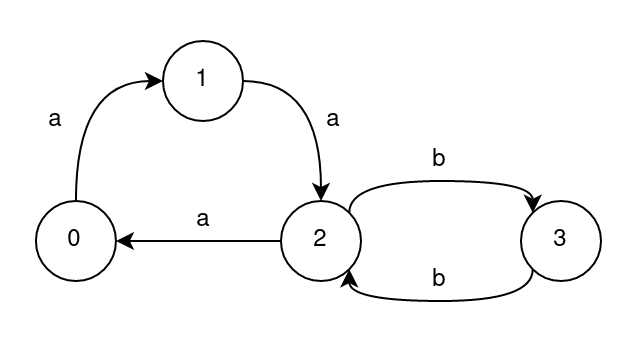
\includegraphics[width=\textwidth]{images/example_graph.png}
%         \caption{Ориентированный граф с меткам}
%     \end{subfigure}
%     \hfill
%     \begin{subfigure}[b]{0.20\textwidth}
%         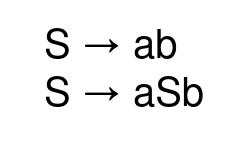
\includegraphics[width=\textwidth]{images/exmample_grammar.png}
%         \caption{Грамматика}
%     \end{subfigure}
%     \caption{Пример графа и грамматики}
% \end{figure}

\subsection{Поиск путей с ограничениями}

При вычислении запроса на поиск путей в графе $\mathcal{G} = \langle V, E, L \rangle$ в качестве ограничения выступает некоторый язык $L$, которому должны удовлетворять результирующие пути.

Поиск путей в графе с семантикой \textbf{достижимости} --- это поиск всех таких пар вершин $(v,u)$, что между ними существует путь $v \pi u$ такой, что $\omega (\pi) \in L$. Результат запроса обозначается как $R = \{ (v,u)~|~\exists v \pi u : \omega (\pi) \in L \}$.

Поиск путей в графе с семантикой \textbf{всех путей} --- это поиск всех таких путей $v \pi u$,   что $\omega (\pi) \in L$. Результат запроса обозначается как $\Pi = \{ v \pi u~|~v \pi u : \omega (\pi) \in L \}$.

Необходимо отметить, что множество $\Pi$ может быть бесконечным, поэтому в качестве результата запроса предполагается не всё множество в явном виде, а некоторый \textit{итератор}, который позволит последовательно извлекать все пути.

Семантика \textbf{одного пути} является ослабленной формулировкой семантики всех путей, так как для получения результата достаточно найти всего один путь вида $v \pi u : \omega (\pi) \in L$ для каждой пары $(v, u) \in R$.

Поскольку язык $L$ может быть бесконечным, при составлении запросов используют не множество $L$ в явном виде, а некоторое правило формирования слов этого языка. В качестве таких правил и выступают регулярные выражения или КС грамматики. При именовании запросов отталкиваются от типа правил, поэтому запросы именуются как регулярные или КС соответственно.

\subsection{Существующие решения}

Впервые проблема выполнения запросов с контекстно-свободными ограничениями была сформулирована в 1990 году в работе Михалиса Яннакакиса~\cite{inproceedings:yannakakis_cfpq_problem}. С того времени были представлены многие работы, в которых так или иначе предлагалось решение данной проблемы. Однако в недавнем исследовании Йохем Куиджперс и др.~\cite{article:kuijpers_cfpq_exp_compare} на основе сравнения нескольких алгоритмов~\cite{article:hellings_cfpq,inproceedings:matrix_cfpq,inbook:santos_cfpq_lr_analysis} для выполнения запросов с контекстно-свободными ограничениями заключили, что существующие алгоритмы неприменимы для анализа реальных данных в силу того, что обработка таких данных занимает значительное время. Стоит отметить, что алгоритмы, используемые в статье, были реализованы на языке программирования \textit{Java} и исполнялись в среде \textit{JVM} в однопоточном режиме, что не является сколь-угодно производительным решением.

Это подтверждают результаты работы~\cite{inproceedings:cfqp_matrix_with_single_source}, в которой с использование программных и аппаратных средств NVIDIA CUDA был реализован алгоритм Рустама Азимова~\cite{inproceedings:matrix_cfpq}. В данном алгоритме задача поиска путей с КС ограничениями для семантики одного пути была сведена к операциям булевой линейной алгебры, что позволило использовать высокопроизводительные библиотеки для выполнения данных операций на GPGPU.

Алгоритм Рустама Азимова~\cite{inproceedings:cfqp_matrix_with_single_source} способен выполнять запросы только в семантике одного пути. Поскольку в качестве формализма для представления грамматики КС запроса используется \textit{нормальная форма Хомского (НФХ)}~\cite{book:automata_theory}, увеличение числа правил в исходной грамматике запроса может приводить к существенному разрастанию НФХ, что негативно влияет на время работы алгоритма.

Недавно представленный алгоритм~\cite{inbook:kronecker_cfpq_adbis} для выполнения КС запросов через произведения Кронекера также использует технику сведения вычислений к операциям булевой алгебры. Однако данный алгоритм позволяет выполнять запросы в семантике всех путей, а также использует в качестве в качестве формализма для представления запроса \textit{рекурсивный автомат}, что потенциально может решить проблему разрастания исходной грамматики запроса.

\subsection{Вычисления на GPGPU}

\textit{GPGPU} (от англ. General-purpose computing on graphics processing units) --- техника использования графического процессора видеокарты компьютера для осуществления неспециализированных вычислений, которые обычно проводит центральный процессор. Данная техника позволяет получить значительной прирост производительности, когда необходимо обрабатывать большие массивы данных с фиксированным набором команд по принципу \textit{SIMD}. 

Исторически видеокарты в первую очередь использовались как графические ускорители для создания высококачественной трехмерной графики в режиме реального времени. Позже стало ясно, что мощность графического процессора можно использовать не только для графических вычислений. Так появились программируемые вычислительные блоки (англ. compute shaders), которые позволяют выполнять на видеокарте неграфические вычисления.

На данный момент существует несколько промышленных стандартов для создания программ, использующих графический процессор, одними из которых являются Vulkan~\cite{net:spec_vulkan}, OpenGL~\cite{net:spec_opengl}, Direct3D~\cite{net:spec_direct3d} как API для графических и неспециализированных вычислительных задач, а также OpenCL~\cite{net:spec_opencl}, NVIDIA CUDA~\cite{net:cuda_toolkit_docs} как API для неспециализированных вычислений. 

В качестве GPGPU в этой работе используется NVIDIA CUDA. В то время как OpenCL создавался как кросс-платформенный стандарт для программирования вычислений, CUDA API специфично только для видеокарт производства компании NVIDIA, однако оно имеет более широкий набор инструментов как для написания, так и для отладки программ, а также собственный компилятор \textit{NVCC}, который позволяет осуществлять кросс-компиляцию кода на языке CUDA, и прозрачно использовать его вместе с кодом на языке C/C++. Кроме этого, в данной работе используется результаты исследования~\cite{inproceedings:cfqp_matrix_with_single_source}, в котором также использовалось CUDA API.

